\newcommand{\anf}[1]{\glqq#1\grqq}
\newcommand{\norm}[1]{\left\|#1\right\|} 
\usetikzlibrary{arrows}

% Zeichenbereich
\tikzstyle{every picture}=[domain=0:4]
% Gitterstil. Zum Stil ’help lines’ wird Linienart ’dotted’ hinzugefügt
\tikzstyle{help lines}+=[dotted]

\begin{frame}{Vektoren - Einführung}
	\begin{center}
		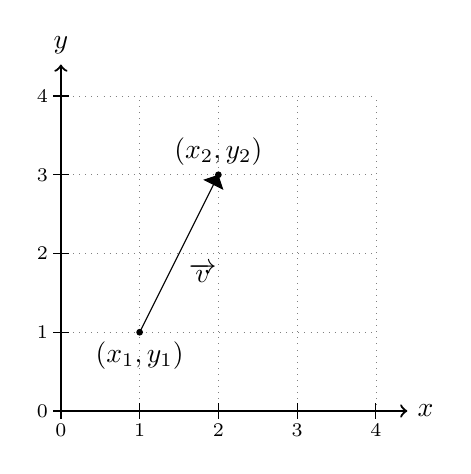
\begin{tikzpicture}[scale=1]
			% Gitter zeichnen
			\draw[style=help lines,step=1cm] (0,0) grid (4,4);
			% Achsen zeichnen
			\draw[->,thick] (-0.1,0) -- (4.4,0) node[right] {$x$};
			\draw[->,thick] (0,-0.1) -- (0,4.4) node[above] {$y$};
			% Punkte zeichnen
			\filldraw (1,1) circle (1pt) node[below] {$(x_1,y_1)$};
			\filldraw (2,3) circle (1pt) node[above] {$(x_2,y_2)$};
			% Vektor zeichnen
			\draw[-triangle 90] (1,1) -- (2,3) node[midway, anchor=north west] {$\overrightarrow{v}$};
			% Achsen beschriften
			\foreach \x in {0,1,2,3,4}
				\draw (\x,-.1) -- (\x,.1) node[below=4pt] {$\scriptstyle\x$};
			\foreach \y in {0,1,2,3,4}
				\draw (-.1,\y) -- (.1,\y) node[left=4pt] {$\scriptstyle\y$};
		\end{tikzpicture}
	\end{center}

	\begin{itemize}
		\item Definiert durch zwei Punkte und eine \anf{Richtung}
		\item $\overrightarrow{v} = \left(\begin{array}{c} x_2 \\ y_2 \end{array}\right) - \left(\begin{array}{c} x_1 \\ y_1 \end{array}\right) = \left(\begin{array}{c} x_2 - x_1 \\ y_2 - y_1 \end{array}\right) = \left(\begin{array}{c} dx \\ dy \end{array}\right)$
	\end{itemize}
\end{frame}

\begin{frame}{Vektoren - Einführung}
	\begin{exampleblock}{Skalieren eines Vektors}
		$\lambda * \overrightarrow{v} := \left(\begin{array}{c} \lambda * x \\ \lambda * y \end{array}\right)$ \\
		Für $\lambda \in (0, 1)$ wird $\overrightarrow{v}$ kürzer,\\
		für $\lambda = 1$ behält $\overrightarrow{v}$ seine Länge bei,\\
		für $\lambda > 1$ wird $\overrightarrow{v}$ länger.
	\end{exampleblock}
	\begin{exampleblock}{Verschieben eines Punktes um einen Vektor}
		$P + \overrightarrow{v} := \left(\begin{array}{c} P_x \\ P_y \end{array}\right) + \left(\begin{array}{c} v_x \\ v_y \end{array}\right) = \left(\begin{array}{c} P_x + v_x \\ P_y + v_y \end{array}\right)$
	\end{exampleblock}
\end{frame}

\begin{frame}{Vektoren - Einführung}
	Skalierung
	\begin{center}
		\begin{tikzpicture}[scale=1]
			% Gitter zeichnen
			\draw[style=help lines,step=1cm] (0,0) grid (4,4);
			% Achsen zeichnen
			\draw[->,thick] (-0.1,0) -- (4.4,0) node[right] {$x$};
			\draw[->,thick] (0,-0.1) -- (0,4.4) node[above] {$y$};
			% Punkte zeichnen
			\filldraw (1,1) circle (1pt);
			% Vektor zeichnen
			\draw[-triangle 90] (1.5,2) -- (2,3) node[midway, anchor=north west] {$\overrightarrow{v}$};
			\draw[draw=red,-triangle 90, fill=red] (1,1) -- (1.5,2) node[midway, anchor=north west] {$\frac{1}{2} * \overrightarrow{v}$};
			% Achsen beschriften
			\foreach \x in {0,1,2,3,4}
				\draw (\x,-.1) -- (\x,.1) node[below=4pt] {$\scriptstyle\x$};
			\foreach \y in {0,1,2,3,4}
				\draw (-.1,\y) -- (.1,\y) node[left=4pt] {$\scriptstyle\y$};
		\end{tikzpicture}
	\end{center}
\end{frame}

\begin{frame}{Vektoren - Einführung}
	Verschiebung
	\begin{center}
		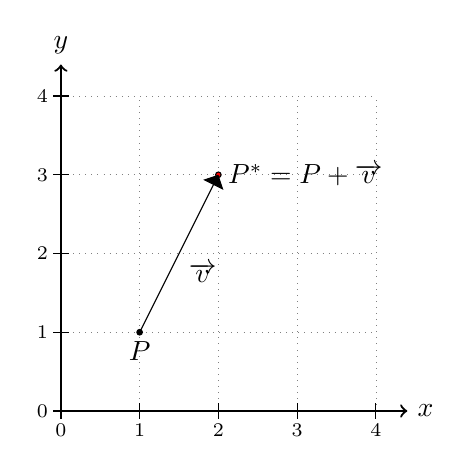
\begin{tikzpicture}[scale=1]
			% Gitter zeichnen
			\draw[style=help lines,step=1cm] (0,0) grid (4,4);
			% Achsen zeichnen
			\draw[->,thick] (-0.1,0) -- (4.4,0) node[right] {$x$};
			\draw[->,thick] (0,-0.1) -- (0,4.4) node[above] {$y$};
			% Punkte zeichnen
			\filldraw (1,1) circle (1pt) node[below] {$P$};
			\filldraw[fill=red] (2,3) circle (1pt) node[right] {$P^* = P + \overrightarrow{v}$};
			% Vektor zeichnen
			\draw[-triangle 90] (1,1) -- (2,3) node[midway, anchor=north west] {$\overrightarrow{v}$};
			% Achsen beschriften
			\foreach \x in {0,1,2,3,4}
				\draw (\x,-.1) -- (\x,.1) node[below=4pt] {$\scriptstyle\x$};
			\foreach \y in {0,1,2,3,4}
				\draw (-.1,\y) -- (.1,\y) node[left=4pt] {$\scriptstyle\y$};
		\end{tikzpicture}
	\end{center}
\end{frame}

\begin{frame}{Vektoren - Einführung}
	\begin{exampleblock}{Länge eines Vektors}
		Die Länge eines Vektors hängt von der verwendeten Norm $\norm{\cdot}$ ab,\\
		überlicherweise verwenden wir die {\bf Euklische Norm} $\norm{\cdot}_2$ .\\
		Im zweidimensionalen Fall ist sie definiert als\\
		$\norm{\left(\begin{array}{c} x \\ y \end{array}\right)}_2 := \sqrt{x^2 + y^2}$
	\end{exampleblock}
\end{frame}

\begin{frame}{Vektoren - Einführung - Code}
	\lstset{
		language=C++,
		tabsize=1
	}
	\lstinputlisting[firstline=1, lastline=14]{vectors.cpp}
\end{frame}

\begin{frame}{Vektoren - Einführung - Code}
	\lstset{
		language=C++,
		tabsize=1
	}
	\lstinputlisting[firstline=16, lastline=29]{vectors.cpp}
\end{frame}

\begin{frame}{Vektoren - Skalarprodukt}
	\begin{exampleblock}{Skalarprodukt zweier Vektoren im kartesischen Koordinatensystem}
		$\left(\begin{array}{c} a_x \\ a_y \end{array}\right) \cdot \left(\begin{array}{c} b_x \\ b_y \end{array}\right) := a_x * b_x + a_y * b_y$
	\end{exampleblock}
	
	Anschaulich betrachtet liefert das Skalarprodukt der Vektoren $\overrightarrow{a}$ und $\overrightarrow{b}$ einen Wert\\
	$< 0$, wenn $\overrightarrow{a}$ und $\overrightarrow{b}$ einen stumpfen Winkel ($> 90^{\circ}$) bilden,\\
	$= 0$, wenn $\overrightarrow{a}$ und $\overrightarrow{b}$ rechtwinklig aufeinander stehen und\\
	$> 0$, wenn $\overrightarrow{a}$ und $\overrightarrow{b}$ einen spitzen Winkel ($< 90^{\circ}$) bilden.
\end{frame}

\begin{frame}{Vektoren - Kreuzprodukt}
	\begin{exampleblock}{Kreuzprodukt zweier Vektoren im zweidimensionalen Fall}
		$\left(\begin{array}{c} a_x \\ a_y \end{array}\right) \times \left(\begin{array}{c} b_x \\ b_y \end{array}\right) := a_x * b_y - a_y * b_x$
	\end{exampleblock}
	
	Das Kreuzprodukt ist normalerweise im dreidimensionalen Raum definiert und liefert einen neuen Vektor, der orthogonal auf beide Vektoren der Eingabe steht.\\
	Im zweidimensionalen Fall liefert das Kreuzprodukt jedoch einen Wert, nämlich die {\bf Z-Koordinate} des Vektors, der senkrecht auf die beiden Vektoren stehen täte.
	Die Länge des neuen Vektors bzw. der Quadrat des Wertes im zweidimensionalen Fall liefert den Flächeninhalt des Parallelogramms, das von den Vektoren $\overrightarrow{a}$ und $\overrightarrow{b}$ aufgespannt wird.
\end{frame}

\begin{frame}{Vektoren - Kreuzprodukt}
	\begin{center}
		(Animation)\\
		Quelle:	\url{http://upload.wikimedia.org/wikipedia/commons/6/6e/Cross_product.gif}
	\end{center}
\end{frame}

\begin{frame}{Vektoren - Skalarprodukt/Kreuzprodukt - Code}
	\lstset{
		language=C++,
		tabsize=1
	}
	\lstinputlisting[firstline=31, lastline=39]{vectors.cpp}
\end{frame}

\begin{frame}{Linksknick-Test/CCW-Test}
	Anhand unserer bisherigen Ergebnisse können wir nun ganz einfach einen Linksknick-Test generieren.
	
	\begin{exampleblock}{}
		\textit{Gegeben:} Drei Punkte $p$, $q$ und $r$.\\
		Bilde die Vektoren $\overrightarrow{pq}$ und $\overrightarrow{pr}$. Berechne das Kreuzprodukt $\tau = \overrightarrow{pq} \times \overrightarrow{pr}$. Der Streckenzug $p \rightarrow q \rightarrow r$ bildet,\\
		falls $\tau < 0$, einen Rechtsknick,\\
		bei $\tau = 0$ sind die Strecken koolinear, und\\
		falls $\tau > 0$, einen Linksknick.\\ \ \\
		
		Wenn also $\tau > 0$ gilt, so ist $p \rightarrow q \rightarrow r$ ein Linksknick.
	\end{exampleblock}
\end{frame}

\begin{frame}{Linksknick-Test/CCW-Test - Code}
	\lstset{
		language=C++,
		tabsize=1
	}
	\lstinputlisting[firstline=41, lastline=49]{vectors.cpp}
\end{frame}

\begin{frame}{Trigonometrie}
	\begin{columns}
	\column{.6\textwidth}
	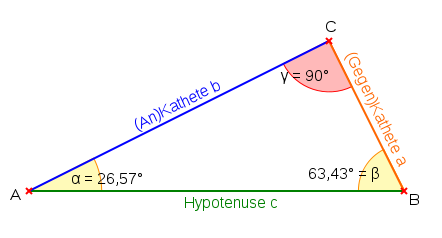
\includegraphics[width=1.1\textwidth,height=.8\textheight,keepaspectratio]{dreieck.png}
	\column{.4\textwidth}
	\begin{itemize}
		\item $\sin \alpha = \frac{Gegenkathete}{Hypotenuse}$
		\item $\cos \alpha = \frac{Ankathete}{Hypotenuse}$
		\item $\tan \alpha = \frac{Gegenkathete}{Ankathete}$
	\end{itemize}
	\end{columns}
	Quelle: \url{http://upload.wikimedia.org/wikipedia/commons/5/56/RechtwinkligesDreieck.svg}
\end{frame}

\begin{frame}{Trigonometrie}
	\begin{center}
		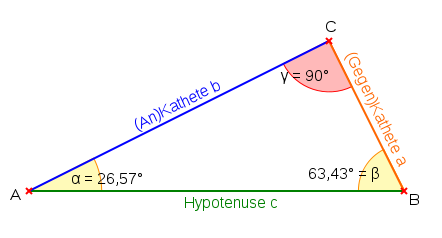
\includegraphics[width=0.6\textwidth,height=.8\textheight,keepaspectratio]{dreieck.png}
	\end{center}
	
	\begin{exampleblock}{Cosinusregel}
		\begin{itemize}
			\item $c^2 = a^2 + b^2 - 2 * a * b * \cos \gamma$
			\item $b^2 = a^2 + c^2 - 2 * a * c * \cos \beta$
			\item $a^2 = b^2 + c^2 - 2 * b * c * \cos \alpha$
		\end{itemize}
	\end{exampleblock}
\end{frame}

\begin{frame}{Trigonometrie}
	\begin{center}
		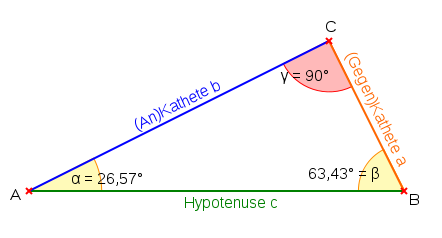
\includegraphics[width=0.6\textwidth,height=.8\textheight,keepaspectratio]{dreieck.png}
	\end{center}
	
	\begin{exampleblock}{Sinusregel}
		$\frac{a}{\sin \alpha} = \frac{b}{\sin \beta} = \frac{c}{\sin \gamma} = \frac{a * b * c}{2 * F}$,
		wobei F der Flächeninhalt des Dreiecks ist.
	\end{exampleblock}
\end{frame}

\begin{frame}{Trigonometrie}
	\begin{exampleblock}{atan2}
		Die Funktion \textit{atan2(y, x)} gibt den Winkel (in RAD) zwischen der x-Achse und dem gegebenen Punkt (x,y) zurück.\\
		Der Wertebereich ist $-\pi < atan2(y, x) \leq pi$.\\
		atan2 ist \textbf{positiv}, wenn die Drehung \textbf{gegen} den Uhrzeigersinn erfolgt, ansonsten \textbf{negativ}.
	\end{exampleblock}
	
	Hinweis: Um von RAD zu DEG zu konvertieren, ist eine Multiplikation mit $\frac{180}{\pi}$ nötig.
\end{frame}